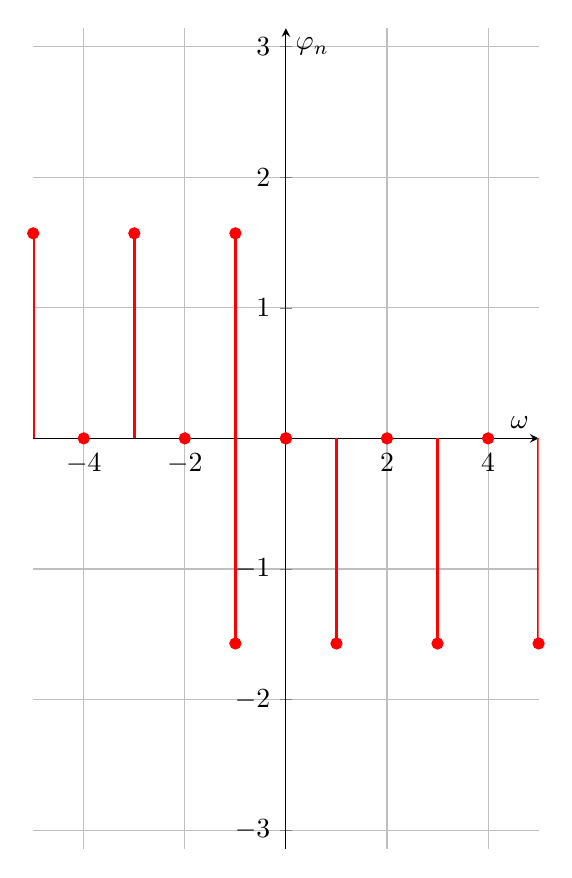
\begin{tikzpicture}
	\begin{axis}[axis lines=middle, grid=both, height=12cm, width=8cm, xmin=-5, xmax=5, ymin=-pi, ymax=pi, xlabel = $\omega$, ylabel = $\varphi_n$]
		\foreach \x in {0,...,5}{
			\addplot[mark=none, red, very thick] coordinates { ({\x * 2 - 1}, 0) ({\x * 2 - 1}, {-pi/2}) };
			\addplot[mark=none, red, very thick] coordinates { ({-\x * 2 - 1}, 0) ({-\x * 2 - 1}, {pi/2}) };
			\addplot[only marks, red] coordinates{ ({\x * 2 - 1}, {-pi/2}) };
			\addplot[only marks, red] coordinates{ ({\x * 2}, {0}) };
			\addplot[only marks, red] coordinates{ ({-\x * 2 - 1}, {pi/2}) };
			\addplot[only marks, red] coordinates{ ({-\x * 2}, {0}) };
		}
	\end{axis}
\end{tikzpicture}